%----------------------------------------------------------------------------------------
%----------------------------------------------------------------------------------------
%----------------------------------------------------------------------------------------
%DATA
%----------------------------------------------------------------------------------------
%----------------------------------------------------------------------------------------
%----------------------------------------------------------------------------------------

\section{DATA}
\label{sec: data}
We use SED templates from K96 to train neural networks.
To test the trained networks, we use SED and physical properties of 142 galaxies at 0.5 < $z$ < 1 from T12.
Following the T12 work, we chose these two sets of data not only to show the application of SOMs in SED clustering, but also to easily compare both supervised and unsupervised methods.

 \subsection{Kinney spectral model}
     \begin{figure}
        \centering
        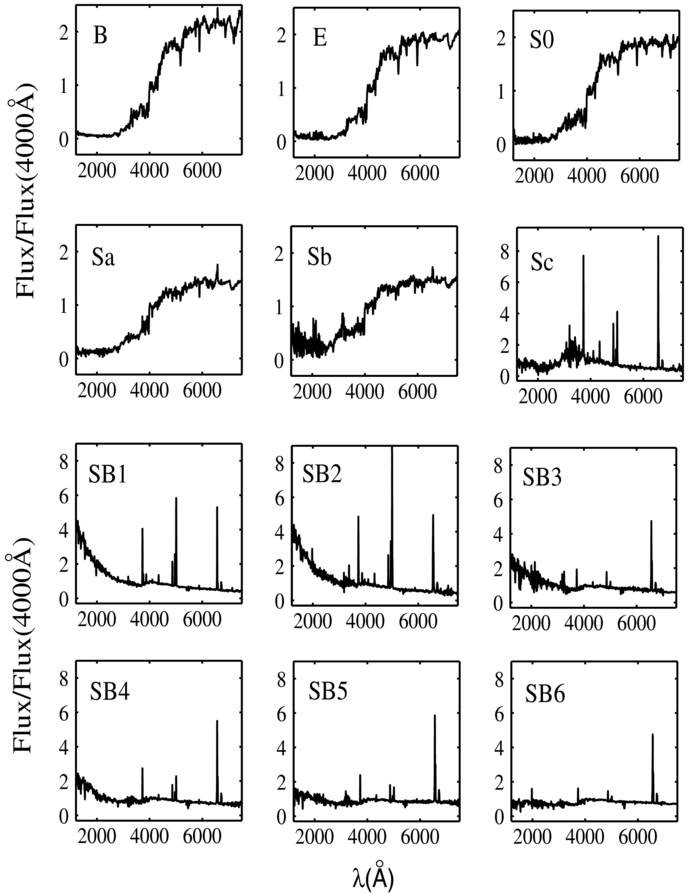
\includegraphics[width=0.5\textwidth]{images/k96.jpg}
        \caption{K96 spectra template for 12 types of galaxies from T12 paper (Fig. 1 in T12). The type of each template is shown in each frame. Plots B, E, S0, Sa, Sb and SC show spectra that belong to the early types galaxies. Starburst galaxies spectra are indicated with SB 1 to 6. Higher numbers represent more intrinsic colour extinction.}
        \label{fig: k96}
    \end{figure}
      
    K96 used UV-optical spectra of 70 star forming and quiescent nearby galaxies to produce a template that contained 12 types of SEDs.
    These templates were widely used in many studies to determine morphological type of galaxies or properties of specific types of galaxies\citep[e.g.][]{Shakouri16,Paiano16,Laporte16,Holden16}.
    K96 claims that these templates can also be used to classifying the SED of the high redshift galaxies. 
    
    The 12 types (what 12 types? the SEDs? in that case this sentence does not belong here at all) of spectra are divided based on their morphological types for early type galaxies or their extinction for starburst galaxies (Fig.~\ref{fig: k96}). 
    The quiescent group of galaxies includes Bulge (B), Elliptical (E), S0, Sa, Sb, and Sc galaxies.
    Bulge group represents galaxies similar to M31 and M81, which their UV and optical spectroscopy is dominated by the stellar population in their bulges.
    The starburst galaxies are divided into six groups (SB1 to SB6) based on their intrinsic extinctions ($E(B-V)$). 
    As it is clear in the Fig.~\ref{fig: k96}, SB1 galaxies have lower internal extinctions ($E(B-V) \simeq 0.05$), while SB6 galaxies have the highest amount of extinction ($E(B-V) \simeq 0.65$) among starburst galaxies. 
    
    K96 spectra spans from $\sim1200$\AA~to $10000$\AA~with a resolution of $\sim 10$\AA.
    However, in this letter we only use data between $\sim1200$\AA ~to $8000$\AA~to train our networks. 
    This wavelength range was chosen due to availability of flux information in those wavelengths for all 12 types of galaxies.
    In early type galaxies' spectra (B to Sb), the spectrum is redder, and strong absorption lines and 4000\AA~break are distinguishable.
    SEDs of starburst galaxies are more flat on the optical and NIR region than those of the the early types and show strong emission lines.
    For more details on each spectral type, we encourage readers to see K96 and references therein. 
    

 \subsection{SED and Properties of the sample galaxies} 
    T12 selected 142 galaxies from the spectroscopic campaign of the ESO GOODS-South field.
    For each galaxy, robust spectroscopic redshift and photometry data from the Good-MUSIC catalogue had been known.
    The 142 galaxies were selected in T12 based on the availability of data from HST/ACS, VLA/ISAAC, and {\it Spitzer}/MIPS and IRAC for whole galaxies. 
    Data from these instruments were necessary in order to have a complete picture of stellar population and SFR.
    The photometry data contain information of the galaxies in 10 - 13 filters with the wavelength range of $\sim 0.4-24~\mu$m in the observed frame.
    T12 matched the resolution of the photometry data with K96 data and used these photometry data as inputs for Code Investigating GALaxy Enmission ({\em CIGALE} code;~\citep[][hereafter N09]{Noll09}) to generate the best fitted SED for each galaxy.% as well as some of the physical properties of the galaxies.
    
    {\em CIGALE} is a valuable tool to investigate the properties of the galaxy using UV to IR wavebands.
    It uses stellar populations, synthetic attenuation and dust emission models, spectral line templates, and active galactic nuclei's optical spectral templates to model SED of the galaxies.
    This code was successfully tested on data from 39 galaxies selected from the Spitzer Infrared Nearby Galaxy Survey (SINGS;~\citep{Kennicutt03}) by N09.
    T12 produced the best SED match, with wavelength interval of 910 to $\sim 8\times10^9$\AA, for each galaxy.
    Assuming decreasing SFR and visual attenuation ($\tau$) model, Salpeter initial mass function~\citep{Salpeter55}, and old stellar population with age of $\sim 10$~Gyr, they derived physical properties of galaxies such as age, and stellar mass.
    Some of these properties are shown in Tab.~\ref{tab: props}.
    In the Sec.~\ref{sec: 1D}, we study these properties for each categorization.
    More details on creating SEDs and extracting information about galaxies properties using {\em CIGALE} can be found in N09 and T12.
    
       
    \begin{table}
\caption[]{Description of the properties of T12 galaxies; the output result of {\em CIGALE}}     
\label{tab: props}
\centering
\begin{tabular}{l l l}
\hline\hline
\noalign{\smallskip}
Par. & Unit & Description\\
\noalign{\smallskip}
\hline
\noalign{\smallskip}
$t_{\,\mathrm{oSP}}$ & Gyr & age of old SP model \\
$t_{\,\mathrm{ySP}}$ & Gyr & age of young SP model \\
$f_\mathrm{burst}$ & --- & mass fraction of \\
& & young single population (SP) model \\
\noalign{\smallskip}
$t_{\,\mathrm{D4000}}$ & Gyr & D4000-related age \\
\noalign{\smallskip}
$M_\mathrm{star}$ & M$_\odot$ & total stellar mass  \\
SFR & M$_\odot$/yr & instantaneous SFR  \\
$A_\mathrm{FUV}$ & mag & attenuation at 1500\,\AA{} \\
\noalign{\smallskip}
\hline
\end{tabular}
\end{table}

    For testing the created networks, we use SEDs that were produced by T12. 
    These SEDs are publicly available in the form of flux per rest frame wavelength in a wide range of wavelengths.
    Since we have used the T12 SEDs to test the trained network, we only used the part of the SEDs that have a same wavelength range as K96 templates.  
 
 %%%%SR160611: The following is the Hossein's answers to the questions that you asked in the data section; Since, we did not used the spectra data here (we only used generated SEDs and information that was derived from SEDs) ,I assumed it is unnecessary to talk a lot about spectroscopy data. But, if you think it would help to understand the subject better, I will add those information to data section.


%  Is the data vector for each object a list of fluxes (flux densities) as a function of (rest) wavelength? I think we discus this question so I skip it.
%  Same wavelengths for every object? Yes
%  What is the spectral resolution? It depends on the type of spectra we use in T12 see
% below for more information.
%  Do the spectra include the whole galaxy or just the central part? For observed 142
% galaxies: whole spectra because they are in high redshift. For K96 they are co-added
% spectra from different parts.
%  Does the resolution match with K96? We match them to K96, see below.
%  What is the coverage of spectra? See below.
%  Do these galaxies have spectroscopic redshifts, or were redshifts derived from
%   photometry?" All 142 galaxies have robust spectroscopic redshift.
% For more clarification about spectra used in T12: We have three sets of spectra.
% 1 – observed spectroscopic spectra. They are used just for extra independent validation; see figure 17 from T12. This validation is nothing to do with network validations. The useful wavelength range (of
% FORS2 spectrometer) is 4800−10 000 Å, the nominal resolution is R = λ/Δλ = 580, which corresponds to
% a spectral resolution of ∼13Å. We use only range [3500-5100] because all the 142 observed spectra have information in this interval (some of them have no spectral information in 8000A, for example). In T12 you can also find this that can help: “The rest-frame spectra of the sample all include spectral information
% ∼3500–5100 Å. This interval brackets the important features such as the 4000Å break and also the strong emission
% lines such as [O ii]λ3727, λHβ 4861, and [O iii] λλ4959, 5007. The spectroscopic data for the sample galaxies contain different spectral types from starbursts (with a flatter continuum and stronger emission lines) to early-type galaxies (with a redder continuum, strong absorption lines, and large 4000Å break.”
% 2- k96 Model spectra which are for training. The spectra cover the interval ∼1200–10000Å and have a resolution of∼10 Å. We use only interval 1200-7500A. because all the 12 K96 spectra have information in
% this interval (some of the spectra have no information in 9000A, for example).
% 3– The Maraston’s models (SEDs): For each galaxy (from 142) we obtain a best Maraston spectrum (SED) by fitting photometric data to the models. Mraston’s models range very extended wavelength interval (from UV to far IR) with different resolution in different part of a given spectrum. For example resolution in IR is 100A and in optical ~3-5A. The best resolution is related to the optical part (3-5A and we convert all to 10A i.e., to resolution of K69). We cut the best 142 spectra in interval [1200-7500] like K96 for ANN validation or test. (If we had spectral information for all K96 spectra in the interval 1200-10000A, for example, then we would cut all 142 SEDs in 1200- 10000A). So if you find a new training set (other than K96 which we talked about that in our skype chat) and if they had information in 1000-15000A, for example, then we would cut the SEDs in this new interval for validation.
% As a summary: as you know (better than me!) we use K96 as training set and 142 SEDs as validation (or test) set. When we obtain the class of each 142 galaxies (in fact 105 galaxies! You are improving this number to 142 in your paper) then we use 105 observed spectra to make figure 17 from T12. The co-added observed spectra in a certain class match with the associated K96 spectra in the same class (i.e., an independent validation).
